

\documentclass[11pt]{article}
\usepackage[utf8]{inputenc}
\usepackage{geometry}
\usepackage{graphicx}
\usepackage{hyperref}
\usepackage{amsmath}
\usepackage{listings}
\usepackage{xcolor}
\usepackage{float}
\usepackage{subcaption}
\usepackage{dirtree}

% Set page margins
\geometry{a4paper, margin=1in}

% Set up code listing style
\lstset{
    basicstyle=\ttfamily,
    commentstyle=\color{gray},
    keywordstyle=\color{blue},
    stringstyle=\color{red},
    showstringspaces=false,
    captionpos=b
}

\title{Development of a Sudoku Solver: C1 Research Computing Coursework}
\author{Vishal Jain}
\date{\today}

\begin{document}

\maketitle

\tableofcontents

\newpage

\section{Introduction}

\begin{quote}
    "Sudoku is a denial of service attack on human
  intellect" - Ben Laurie
\end{quote}

This report details the development of a Sudoku solver inline with the requirements of the C1 Research Computing coursework. The programme takes as input an incomplete grid in the form of a text file with a 9x9 grid of numbers with zero representing unknown values and `|`,`+`,`-` separating cells and , i.e.:


\begin{verbatim}
    $ cat input.txt
    000|007|000
    000|009|504
    000|050|169
    ---+---+---
    080|000|305
    075|000|290
    406|000|080
    ---+---+---
    762|080|000
    103|900|000
    000|600|000
    \end{verbatim}

and outputs the completed grid in the same form.


\section{Problem Decomposition}
To architect the Sudoku solver program, an initial flowchart was constructed to map out the high-level logical sequence. Each step of the flowchart was assigned a color based on its logical independence. This method helped identify distinct, modular components within the program's workflow. The resulting color-coded flowchart is presented in Figure \ref{fig:solver_flowchart}.


The analysis led to the identification of the following key modular components in the Sudoku solver:

\begin{itemize}
\item \textbf{User IO:} Handles user interaction and input/output processing.
\item \textbf{Format Validation:} Ensures the correctness of the input format.
\item \textbf{Board Logic:} Converts input Sudoku boards into a standardised internal format suitable for efficient manipulation.
\item \textbf{Solver Logic:} Implements the algorithms to solve the Sudoku puzzle.
\end{itemize}


\subsection{Developmental Journey}
Before delving into the final structure of the Sudoku solver, it is insightful to explore the initial prototyping phase. This phase laid the groundwork for the project and provided key insights that shaped the final design.

\begin{figure}[H]
\centering
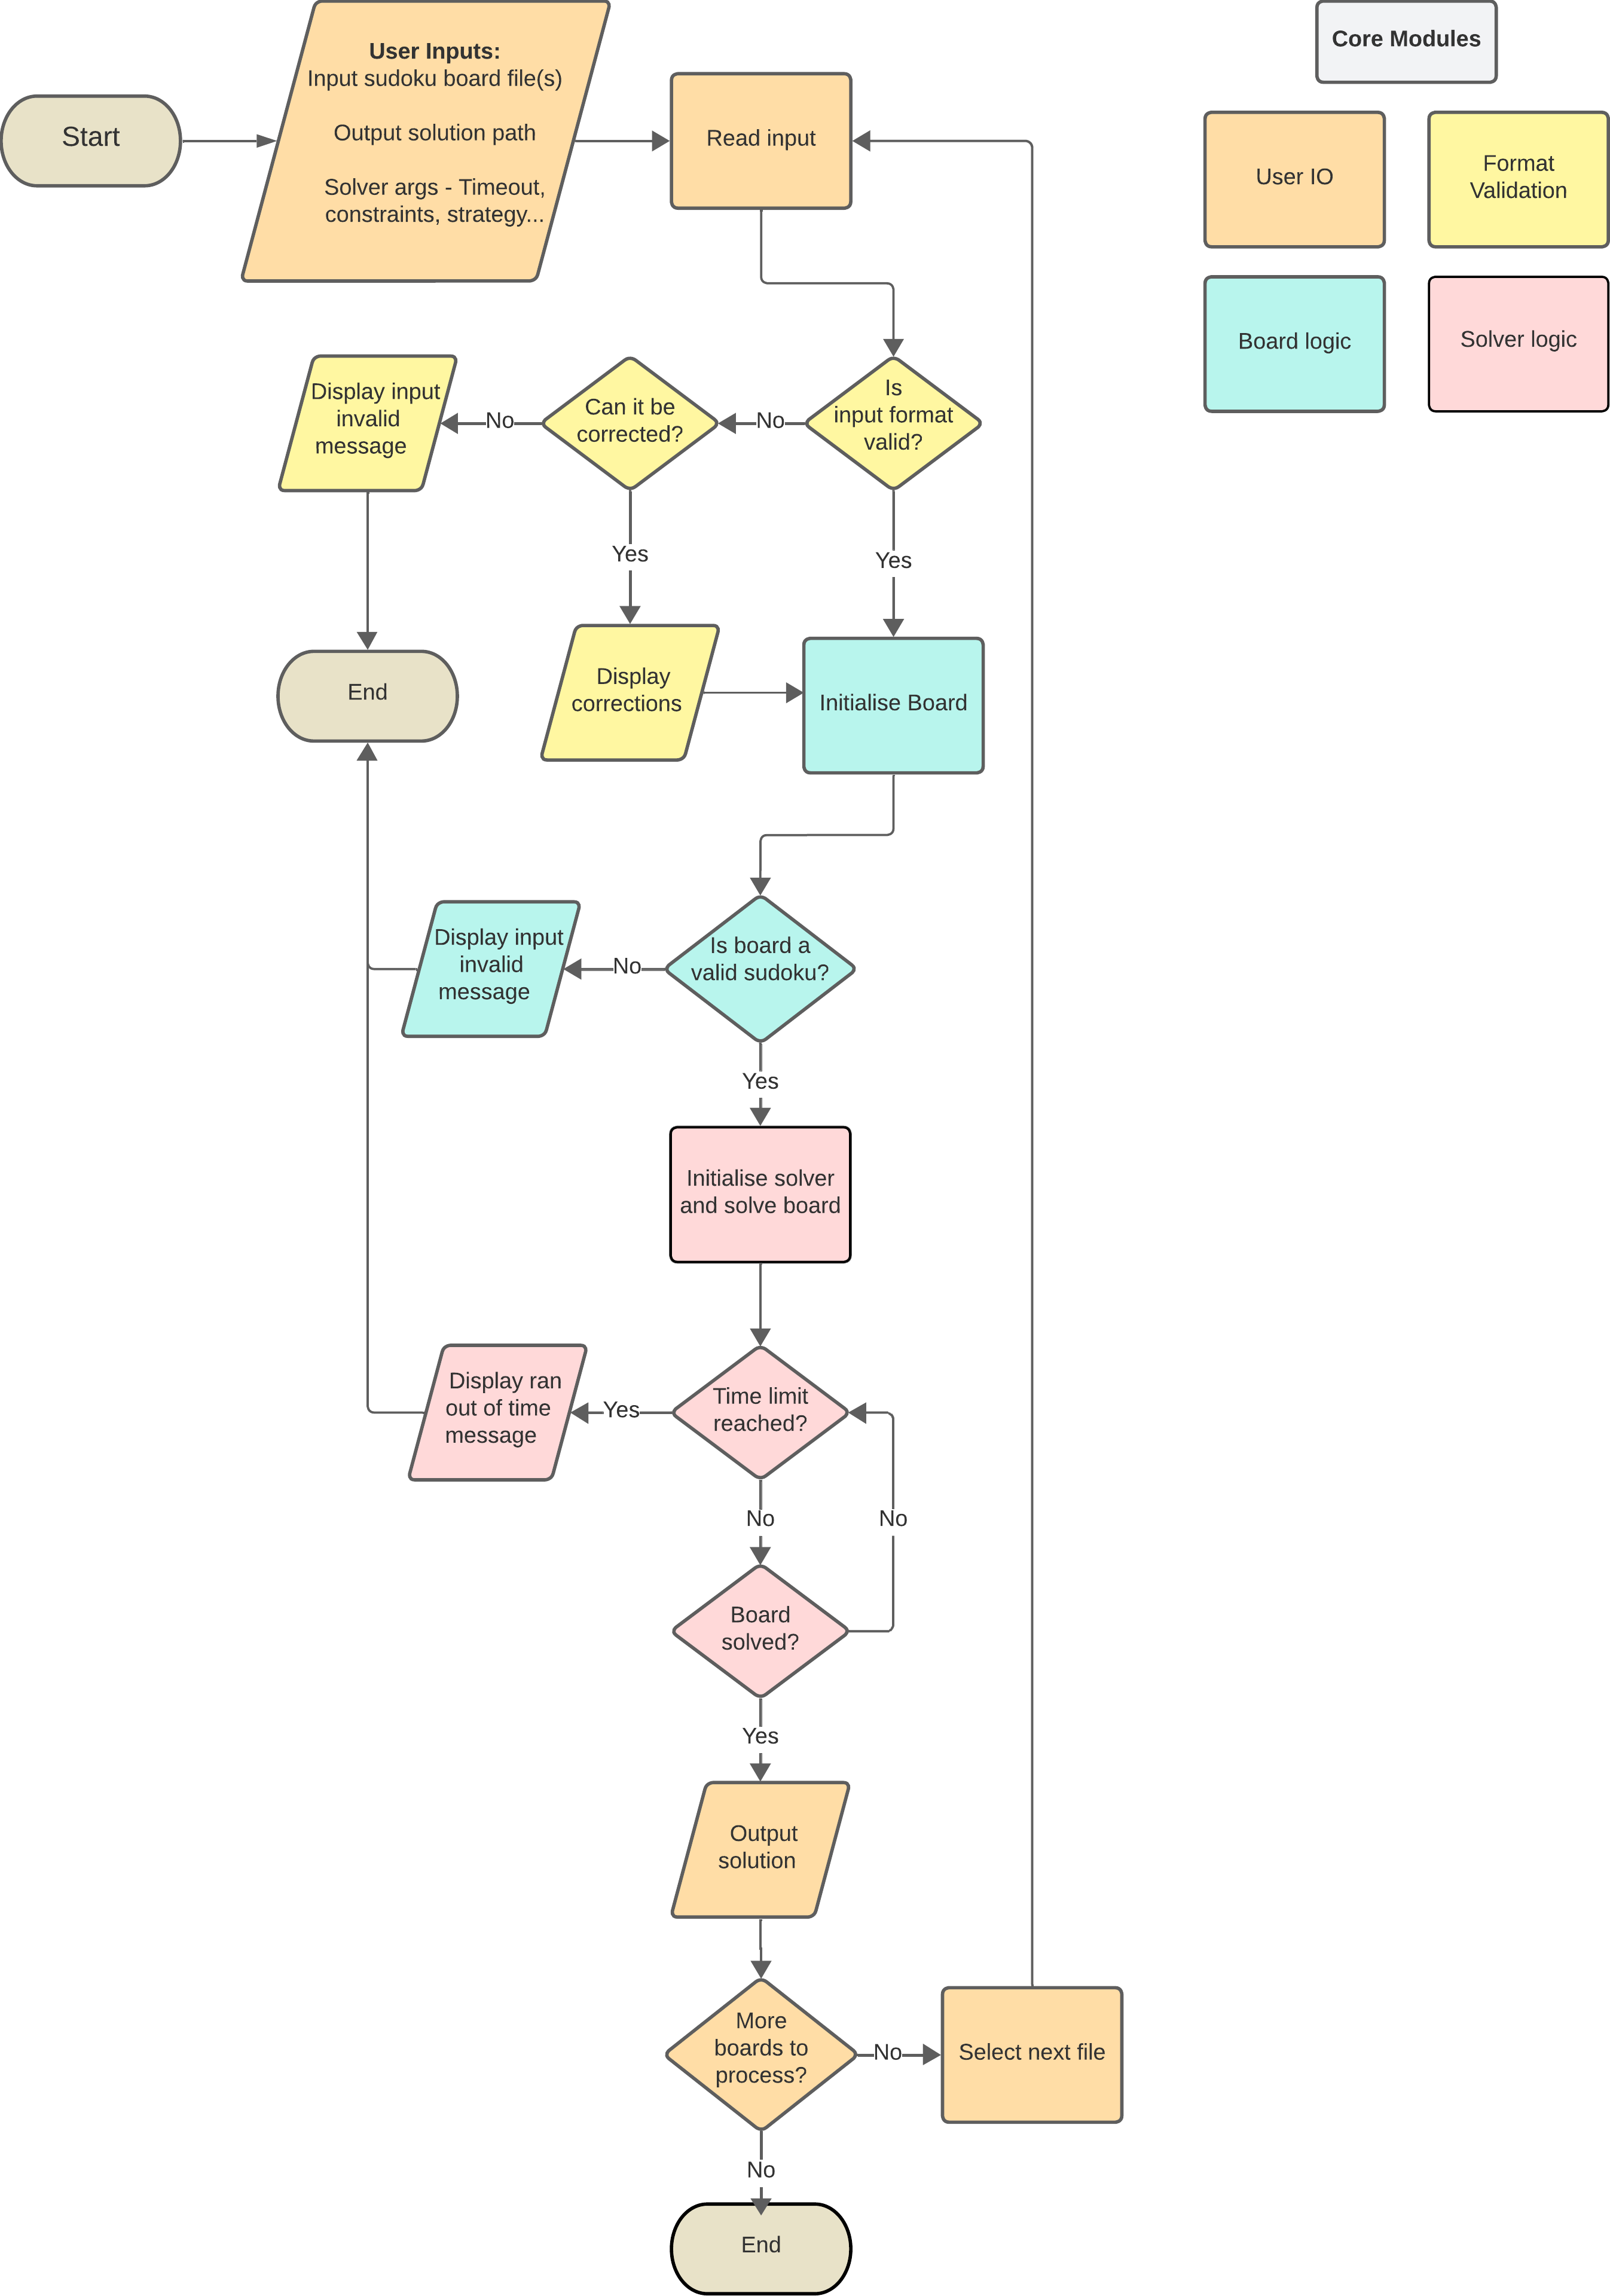
\includegraphics[width=1\textwidth]{figs/solver_flowchart.png}
\caption{High-level flowchart of the Sudoku solver program, illustrating the initial conceptual design. Related pieces of logic are color-coded: orange for user interaction, yellow for format validation, cyan for board logic and pink for solver related logic.}


\label{fig:solver_flowchart}
\end{figure}

\subsubsection{Early Prototyping}
In the initial stages, the envisioned usage of the program was conceptualised as a straightforward sequence of operations involving board validation, board representation, solving and saving. The logical flow was as follows:

\begin{enumerate}
\item \textbf{Board Validation}: The user provides a file containing the Sudoku puzzle, which is then read, validated, and corrected if necessary. This process was handled by a utility function, \texttt{validate\_board}, located in the \texttt{utils} module. The function's purpose was to ensure the input adhered to Sudoku format standards and to correct any discrepancies. The code snippet for this step:
\begin{verbatim}
board_array = utils.validate_board(board_file)
\end{verbatim}
This function returns a 9x9 numpy array representing the initial state of the Sudoku board.

\item \textbf{Board Representation}: The returned board array is then used to initialise an instance of the `\texttt{SudokuBoard}` class. This class encapsulates the board's representation and manipulation logic, offering standard board operations such as `\texttt{reset}` and `\texttt{check\_valid}`. The initialisation step is shown below:
\begin{verbatim}
board = SudokuBoard(board_array)
\end{verbatim}

\item \textbf{Solving the Puzzle}: The next step involved passing the \texttt{SudokuBoard} instance to the \texttt{solve} method of the solver class. This returned a new `\texttt{SudokuBoard}` instance representing the solved board:
\begin{verbatim}
solved_board = Solver(board).solve()
\end{verbatim}
The details of the specific solver used will be discussed in a later section.

\item \textbf{Puzzle Saving}: The final step was to save the solution in the original format. This functionality is encapsulated in the board.save() method of the \texttt{SudokuBoard} class. 
\begin{verbatim}
solved_board.save(save_path)
\end{verbatim}
\end{enumerate}

\subsubsection{Early Hurdles and Insights}

Benchmarking the initial prototype against a Kaggle dataset revealed several design and functionality challenges:

\begin{itemize}
\item \textbf{Format Handling Limitation:} The primary obstacle was accommodating different input formats. Rather than resort to makeshift conversion scripts, it became clear that a sustainable approach was to develop a comprehensive format handling framework, ensuring native support for diverse input formats and streamlining the addition of new ones.

\item \textbf{Validation Logic Overload:} The \texttt{validate\_board} function grew cumbersome as it handled more validation and correction logic, straying from the principles of single responsibility and modularity.

\item \textbf{Misplaced Save Method:} In the context of supporting multiple formats, it was logical to transfer the \texttt{save} method from the \texttt{SudokuBoard} class to the format classes where the custom parsing methods would be defined as saving and parsing are two sides of the same coin and should live together.

\item \textbf{Solver Framework Incompleteness:} The solver class lacked a clear framework which was capable of for incorporating alternative algorithms, hindering the dynamic selection and testing of various solving strategies on the same dataset.

\item \textbf{Lack of Back-End Abstraction in Main:} The inflexibility of the \texttt{main.py} module became apparent, as integrating new format handlers or solvers necessitated direct modifications to the front end script, going against the principles of modularity and encapsulation.

\item \textbf{Main Script Inflexibility:} The inability to process directories of board files limited batch testing capabilities. Moreover, the need to support string inputs for swift testing became apparent. 
\end{itemize}

\subsubsection{High-Level Overview of the Final Implementation}
The final design of the Sudoku solver program encapsulates a modular and flexible architecture, as outlined below:

\begin{verbatim}
# Initialise the Format Handler and Solver
format_handler = SudokuFormatHandler()
solver = SudokuSolver()

# Parse the Sudoku board from the given input in the desired format
board = format_handler.parse(board_file, format_type)

# Employ a specific solver to find a solution for the parsed board 
solved_board = solver.solve(board, solver_backend)

# Save the solved board in the desired format and output path
format_handler.save(solved_board, format_type, output_path)
\end{verbatim}

In this design, \texttt{SudokuFormatHandler} and \texttt{SudokuSolver} act as wrapper classes. Their methods accept parameters which allow the user to specify the desired format and solver backend. The corresponding arguments for these parameters are collected by the \texttt{main.py} script. The next section will explore the design and implementation of the various modules in greater detail.

\section{Programme Modules}
\subsection{SudokuFormatHandler Class}

\subsubsection{Scope}
The scope of format handler classes, as implemented in \texttt{sudoku\_format\_handlers.py}, is defined by their role in bridging the external representations of Sudoku boards and their standardised internal representations. In this context, their scope includes:

\begin{itemize}
\item \textbf{Parsing}: Handling the conversion of the input, whether it comes as a string or as a file path, into a standardised \texttt{SudokuBoard} object.

\item \textbf{Saving}: Conversely, the class also manages the conversion of \texttt{SudokuBoard} objects back into user-readable formats. 

\item \textbf{Format Validation and Correction}: This class is also where the developer defines any methods for validation checks and corrections to ensure that the input is in the expected format before parsing.
\end{itemize}

\subsubsection{Design and Implementation}
The design of the module is such that there is a central \texttt{SudokuFormatHandler} class which calls the other implemented \texttt{FormatHandler} classes. This approach is centered on the principles of modularity and extensibility, driven by the use of an abstract base class and a handler dictionary. Key design aspects include:

\begin{itemize}
    \item \textbf{Modularity}: The class leverages an abstract base class, \texttt{FormatHandler}, which outlines essential methods -- \texttt{parse} and \texttt{save}. This structure ensures consistency across different format handlers while allowing for flexibility in their specific implementations.
    \item \textbf{Extensibility}: New formats can be easily integrated into the system by creating a subclass of \texttt{FormatHandler} and adding it to \texttt{SudokuFormatHandler}'s \texttt{handler\_dict} class attribute. This new format will automatically be made available for selection through the \texttt{main.py} script. 
\end{itemize}
The UML class diagrams in Figure \ref{fig:format_handler_uml} provide a visual representation of the design and implementation of the \texttt{FormatHandler} abstract base class and the concrete grid and line format handler classes used by the \texttt{SudokuFormatHandler} class.

\begin{figure}[H]
    \centering
    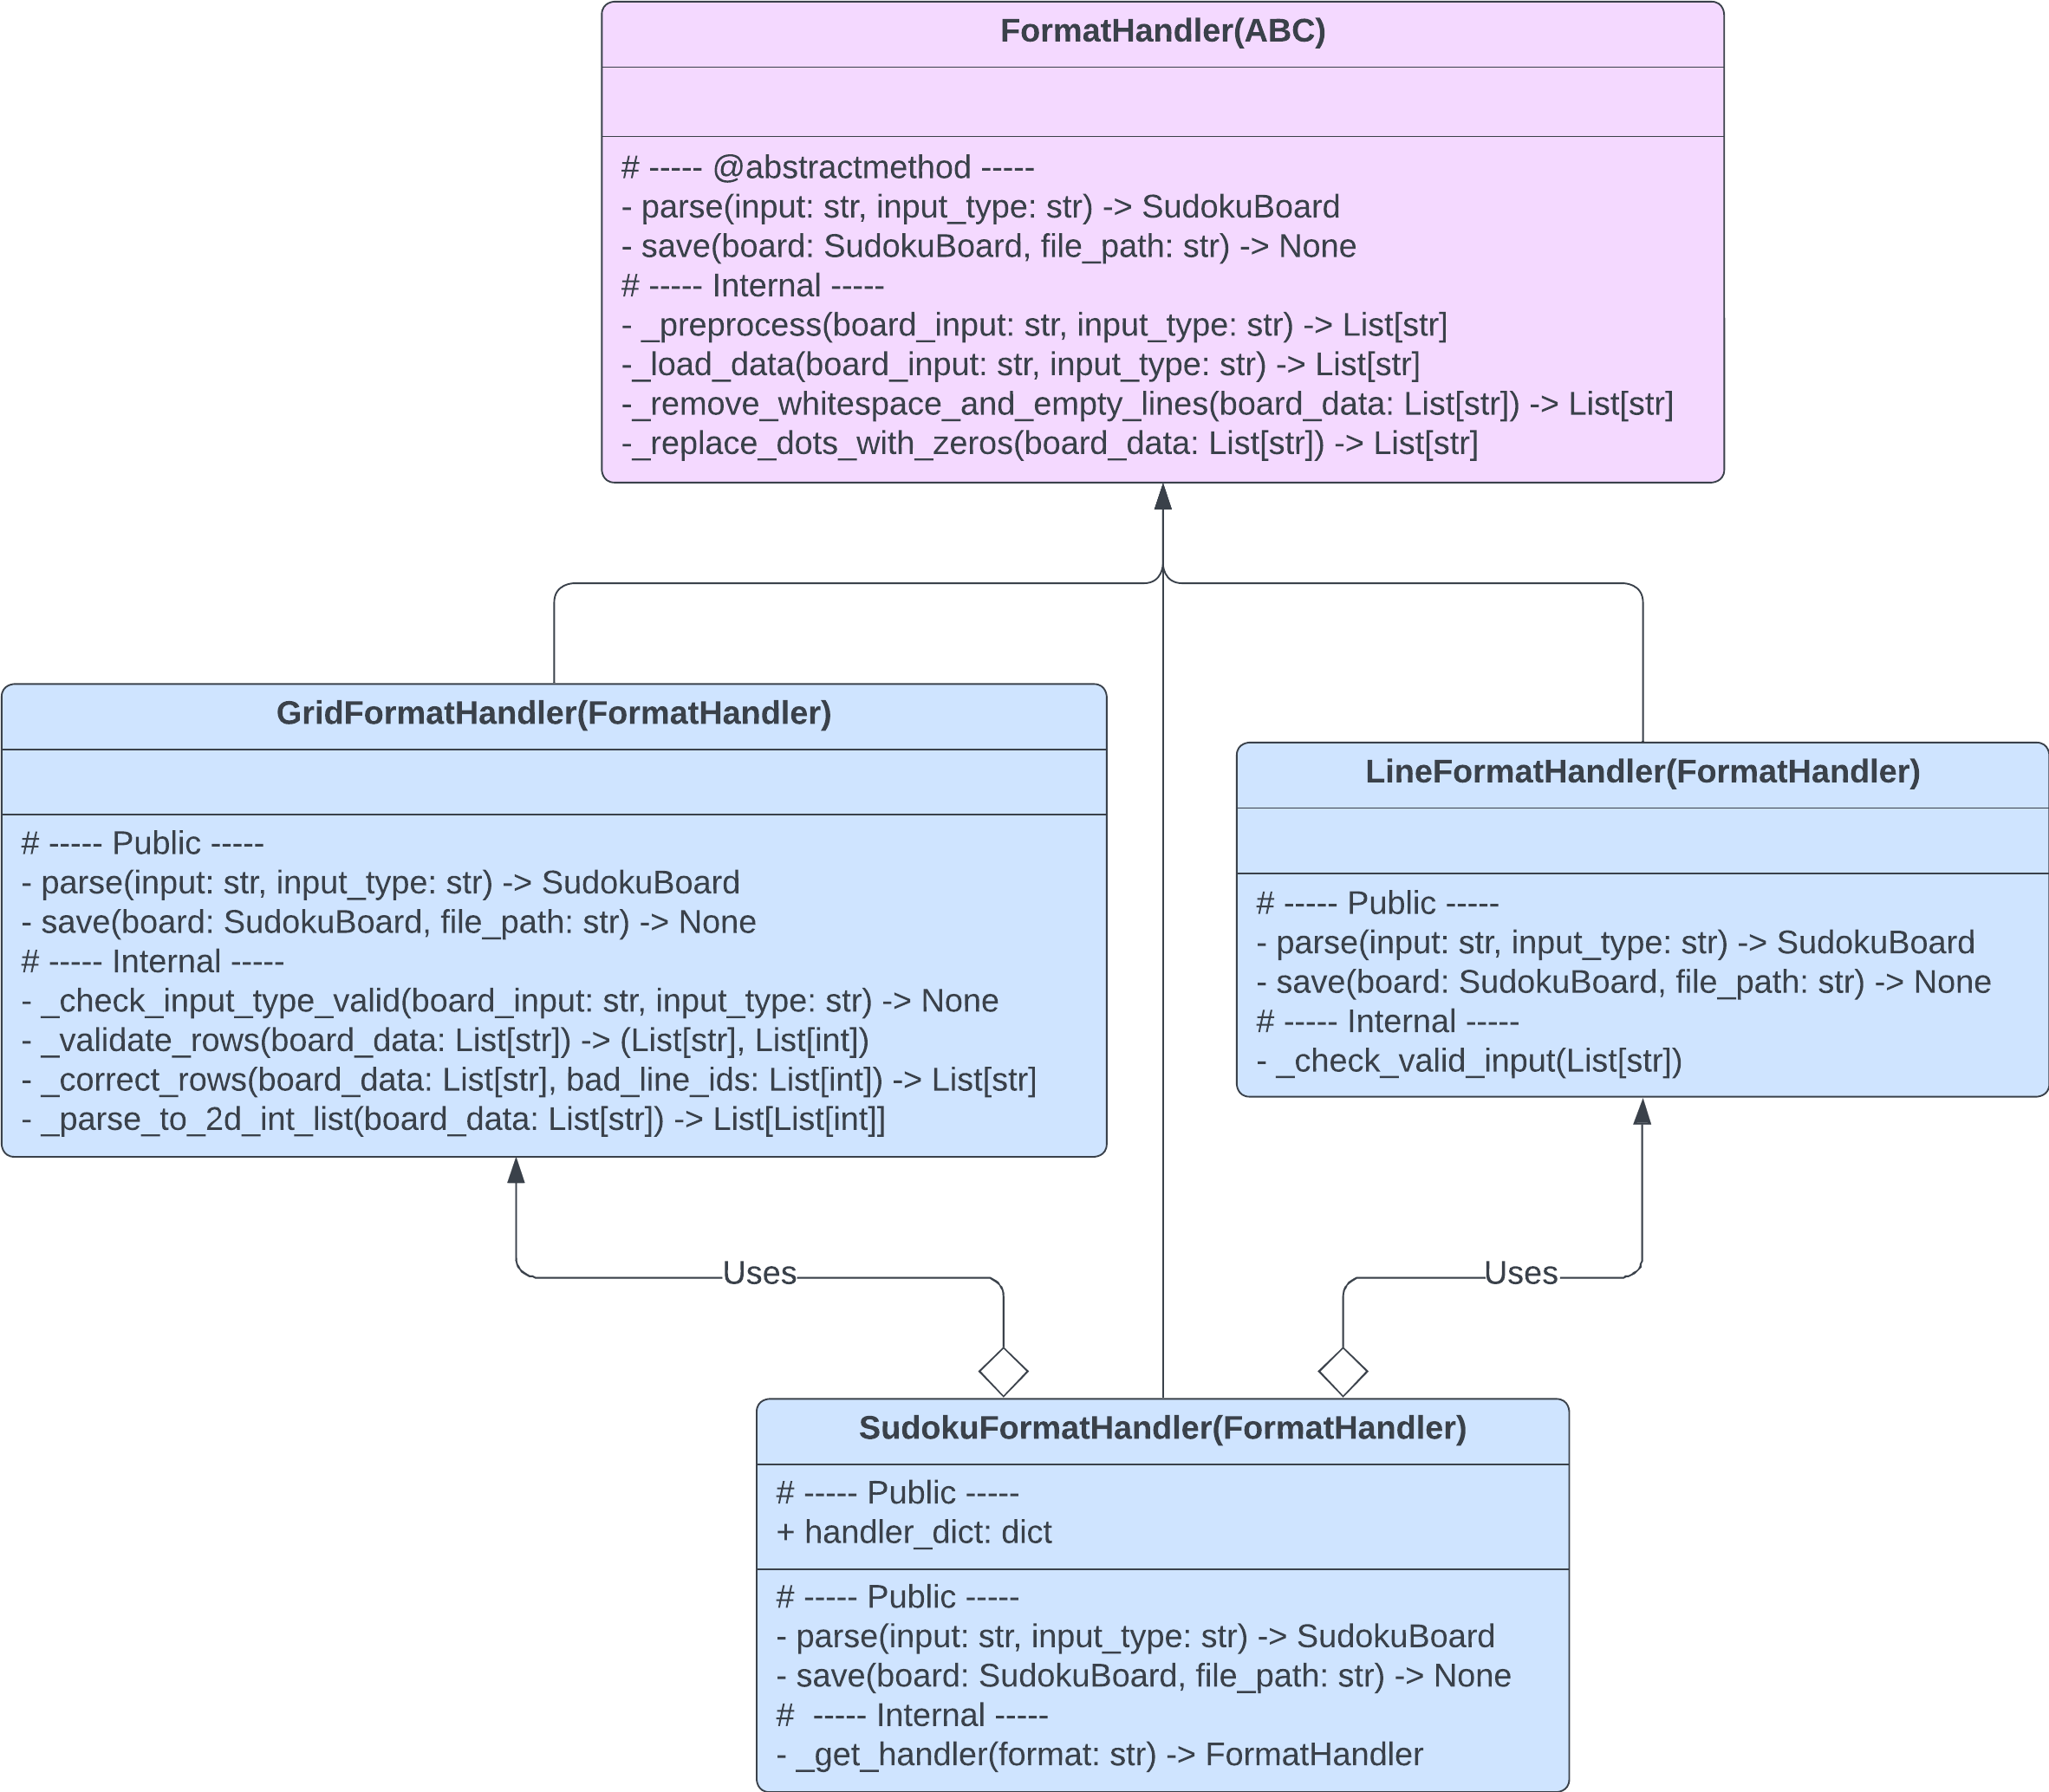
\includegraphics[width=1\textwidth]{figs/UML_sudoku_handlers.png}
    \caption{UML class diagram for implementation of the FormatHandler classes. Abstract classes are depicted in pink, concrete classes in blue. Composition relationships are indicated with arrows having a white diamond base and a solid head.}
    \label{fig:format_handler_uml}
\end{figure}

\paragraph{GridFormatHandler}
The GridFormatHandler is the format handler for the required format of this coursework. It is designed to handle the parsing and saving of Sudoku boards in the grid format. The parsing process involves reading the input file or string and converting it into a list of strings representing each row of the Sudoku board. The white space and empty lines are removed. Any dots are replacecd with zeros as this is commonly seen online as a placeholder for empty cells. The handler ensures there are exactly 11 rows; otherwise, it raises an error. Each row undergoes validation against a specific regex pattern. If a row deviates from the expected pattern but aligns with an alternate acceptable one, it undergoes correction; otherwise, an error is raised. Correction logic is applied selectively: separator rows lacking numbers are replaced with a standard separator row, but if they contain numbers, an error is raised to avoid digit alteration. For a row which is expected to describe a number row, if it matches the general pattern of 3 sets of numeric character triplets seperated by a non numeric character, it is corrected by inserting the expected seperator characters between the triplets.
\subsubsection{Limitations}
The module's primary limitation lies in its capability to process only a single Sudoku board per file, rather than supporting multiple boards in one file. This is not an oversight but a deliberate design choice. Accommodating multi-board parsing from a single file can substantially escalate the complexity of the classes. This is because the way you can specify multiple boards is unique to each format. For instance, in the grid format, multiple boards can be specified by separating them with a blank line. However, in the line format, multiple boards can be specified by separating them with a comma. Further, the complexity of the validation logic would also increase. Development of a format handling system that is capable of robustly handling such variability falls outside the scope of this coursework.


\subsection{SudokuBoard Class}

\subsubsection{Scope}
The \texttt{SudokuBoard} class defined in \texttt{sudoku\_board.py} is integral to the overall programme, providing a standardised interface for the other classes. The scope of this class encompasses:

\begin{itemize}
    \item \textbf{Board Representation}: Providing an internal representation of a Sudoku board. 
    \item \textbf{Board Validation}: Making sure the board state always describes a valid Sudoku.  
    \item \textbf{Board Manipulation}: Implementing methods for  efficient manipulation and access of the board state.
\end{itemize}
\subsubsection{Design and Implementation}
The design of the \texttt{SudokuBoard} class adheres to the principle of encapsulation, ensuring that the internal state of the board is managed in a controlled manner. 
\begin{itemize}
\item \textbf{Efficient Board Representation}: The class uses a 2D numpy array for board representation, enhanced with lists of sets to track the state of the rows, columns, and subgrids.  Leveraging the speed of numpy arrays and the fast lookup capabilities of sets for validating and managing the board state.
\item \textbf{Controlled and Encapsulated Board Interaction}: The class maintains encapsulation, offering array-like read-only access via the \texttt{\_\_getitem\_\_} method, while preventing direct board modifications. Controlled manipulation is facilitated through specific methods like \texttt{place\_number} and \texttt{remove\_number}, ensuring adherence to Sudoku rules and maintaining the integrity of the board's state.

\item \textbf{Convenience Methods}: The class offers various utility methods such as resetting the board and finding empty cells. These methods simplify common operations required for solving Sudoku puzzles.

\item \textbf{Initialisation with Integrated Validation}: The \texttt{\_\_init\_\_} method performs an immediate validation check of the board state, confirming adherence to Sudoku rules upon setup.

\item \textbf{Board Formatting for Debugging and Visualisation}: The \texttt{\_\_str\_\_} method formats the board into a human-readable string, aiding in debugging and visualisation.
\end{itemize}

The UML class diagram in Figure \ref{fig:sudoku_board_uml} provides a visual representation of the implementation of the \texttt{SudokuBoard} class.

\begin{figure}[H]
    \centering
    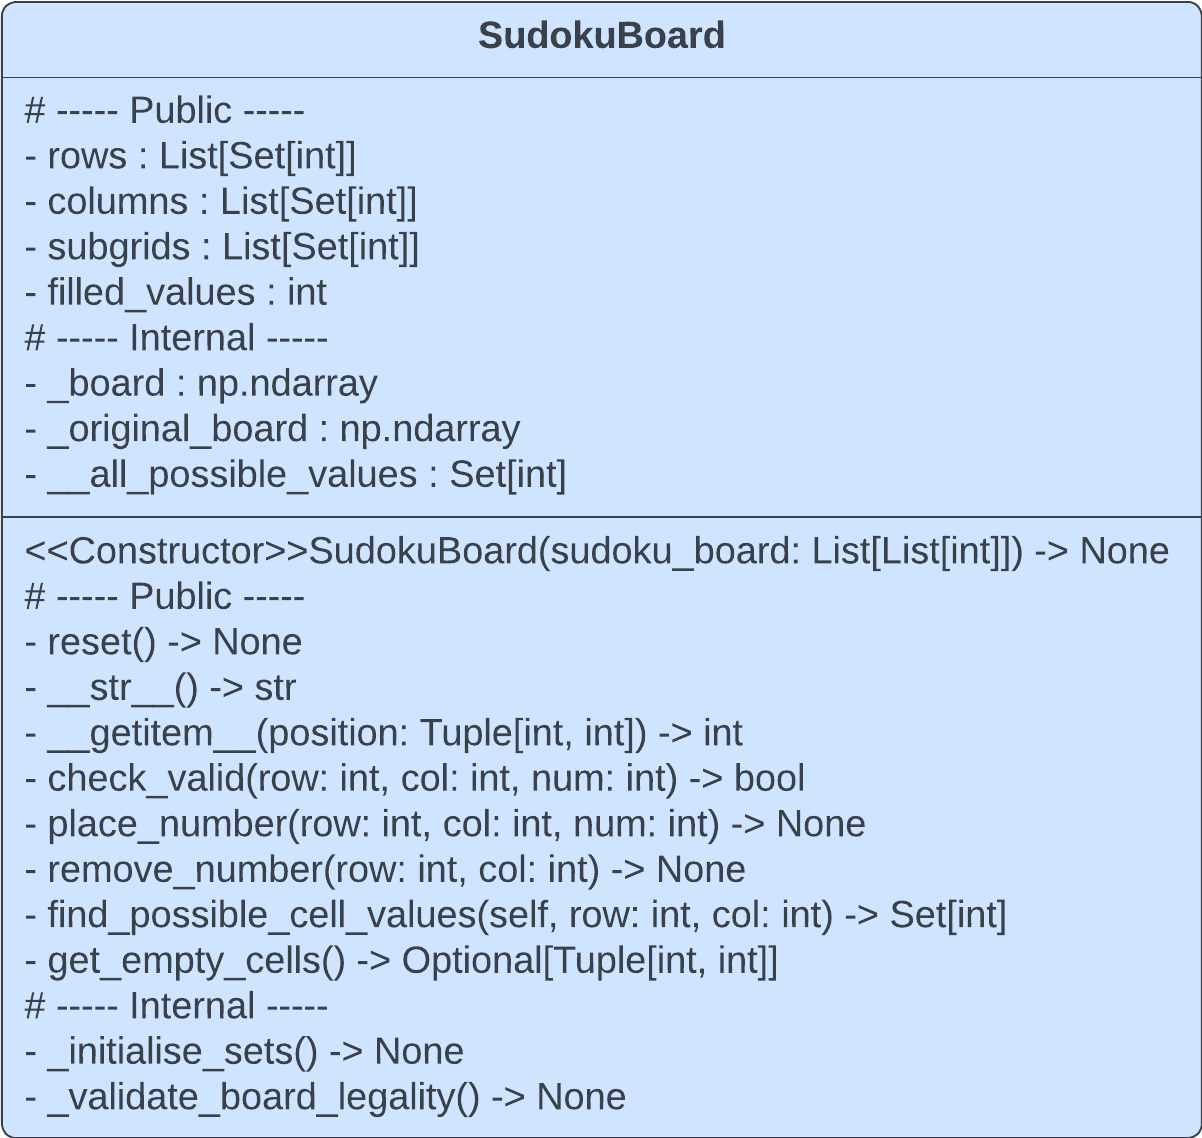
\includegraphics[width=0.6\textwidth]{figs/UML_sudoku_board.png}
    \caption{UML class diagram for the SudokuBoard module.}
    \label{fig:sudoku_board_uml}
\end{figure}
 
\subsubsection{Limitations}
The \texttt{SudokuBoard} class, unlike \texttt{SudokuFormatHandler}, isn't inherently extensible for different board types such as dictionary representations often used in more optimised solvers. To address this, an abstract \texttt{Board} base class could be introduced, defining the common methods for solvers and format handlers with their expected inputs and outputs. \texttt{SudokuBoard} would then act as a wrapper class, instantiating the specific concrete \texttt{Board} implementations specified by the user.


\subsection{SudokuSolver Class}
\subsubsection{Scope}
The scope of solver classes, as implemented in \texttt{sudoku\_solvers.py}
is defined by the following:
\begin{itemize}
    \item \textbf{Solving}: Taking in a \texttt{SudokuBoard} object and returning a solved \texttt{SudokuBoard} object.
    \item \textbf{Outputting Solve Status}: Returning the status of the solution.
\end{itemize}

\subsubsection{Theory - Backtracking}
The type of solver implemented in this coursework is based on the method of backtracking. Backtracking is a brute-force method that uses recursive depth-first search to explore all possible solutions, starting from the initial state of the Sudoku board. This method systematically tries every valid option for each empty cell and backtracks when it reaches a state where it can't make any valid moves. While this method is comprehensive, it can be inefficient on some boards due to its lack of strategic direction in cell selection. To enhance this approach, an additional version incorporating a heuristic to prioritise cells with the fewest possible values, reducing the number of possibilities to explore. Both these approaches are implemented in the Sudoku solver program as \texttt{BacktrackingSolverBasic} and \texttt{BacktrackingSolverEasiestFirst} respectively. Their performances are compared in a later section.
\subsubsection{Design and implementation}
\begin{itemize}
    \item \textbf{Modularity}: The class leverages an abstract base class, \texttt{Solver}, which outlines the essential method for all solvers -- \texttt{solve}. This structure ensures consistency across different solvers while allowing for flexibility in their specific implementations.
    \item \textbf{Extensibility}: New solvers can be easily integrated into the system by creating a subclass of \texttt{Solver}. After implementation, they can be added to \texttt{SudokuSolvers}'s \texttt{solver\_dict} class attribute. They will automatically be available for selection through the \texttt{main.py} script.
\end{itemize}

The UML class diagrams in Figure \ref{fig:sudoku_solver_uml} provide a visual representation of the design and implementation of the \texttt{Solver} abstract base class and the \texttt{SudokuSolver} class along with the implemented \texttt{BacktrackingSolverBasic} and {BacktrackingSolverEasiestFirst} classes.

\begin{figure}[H]
    \centering
    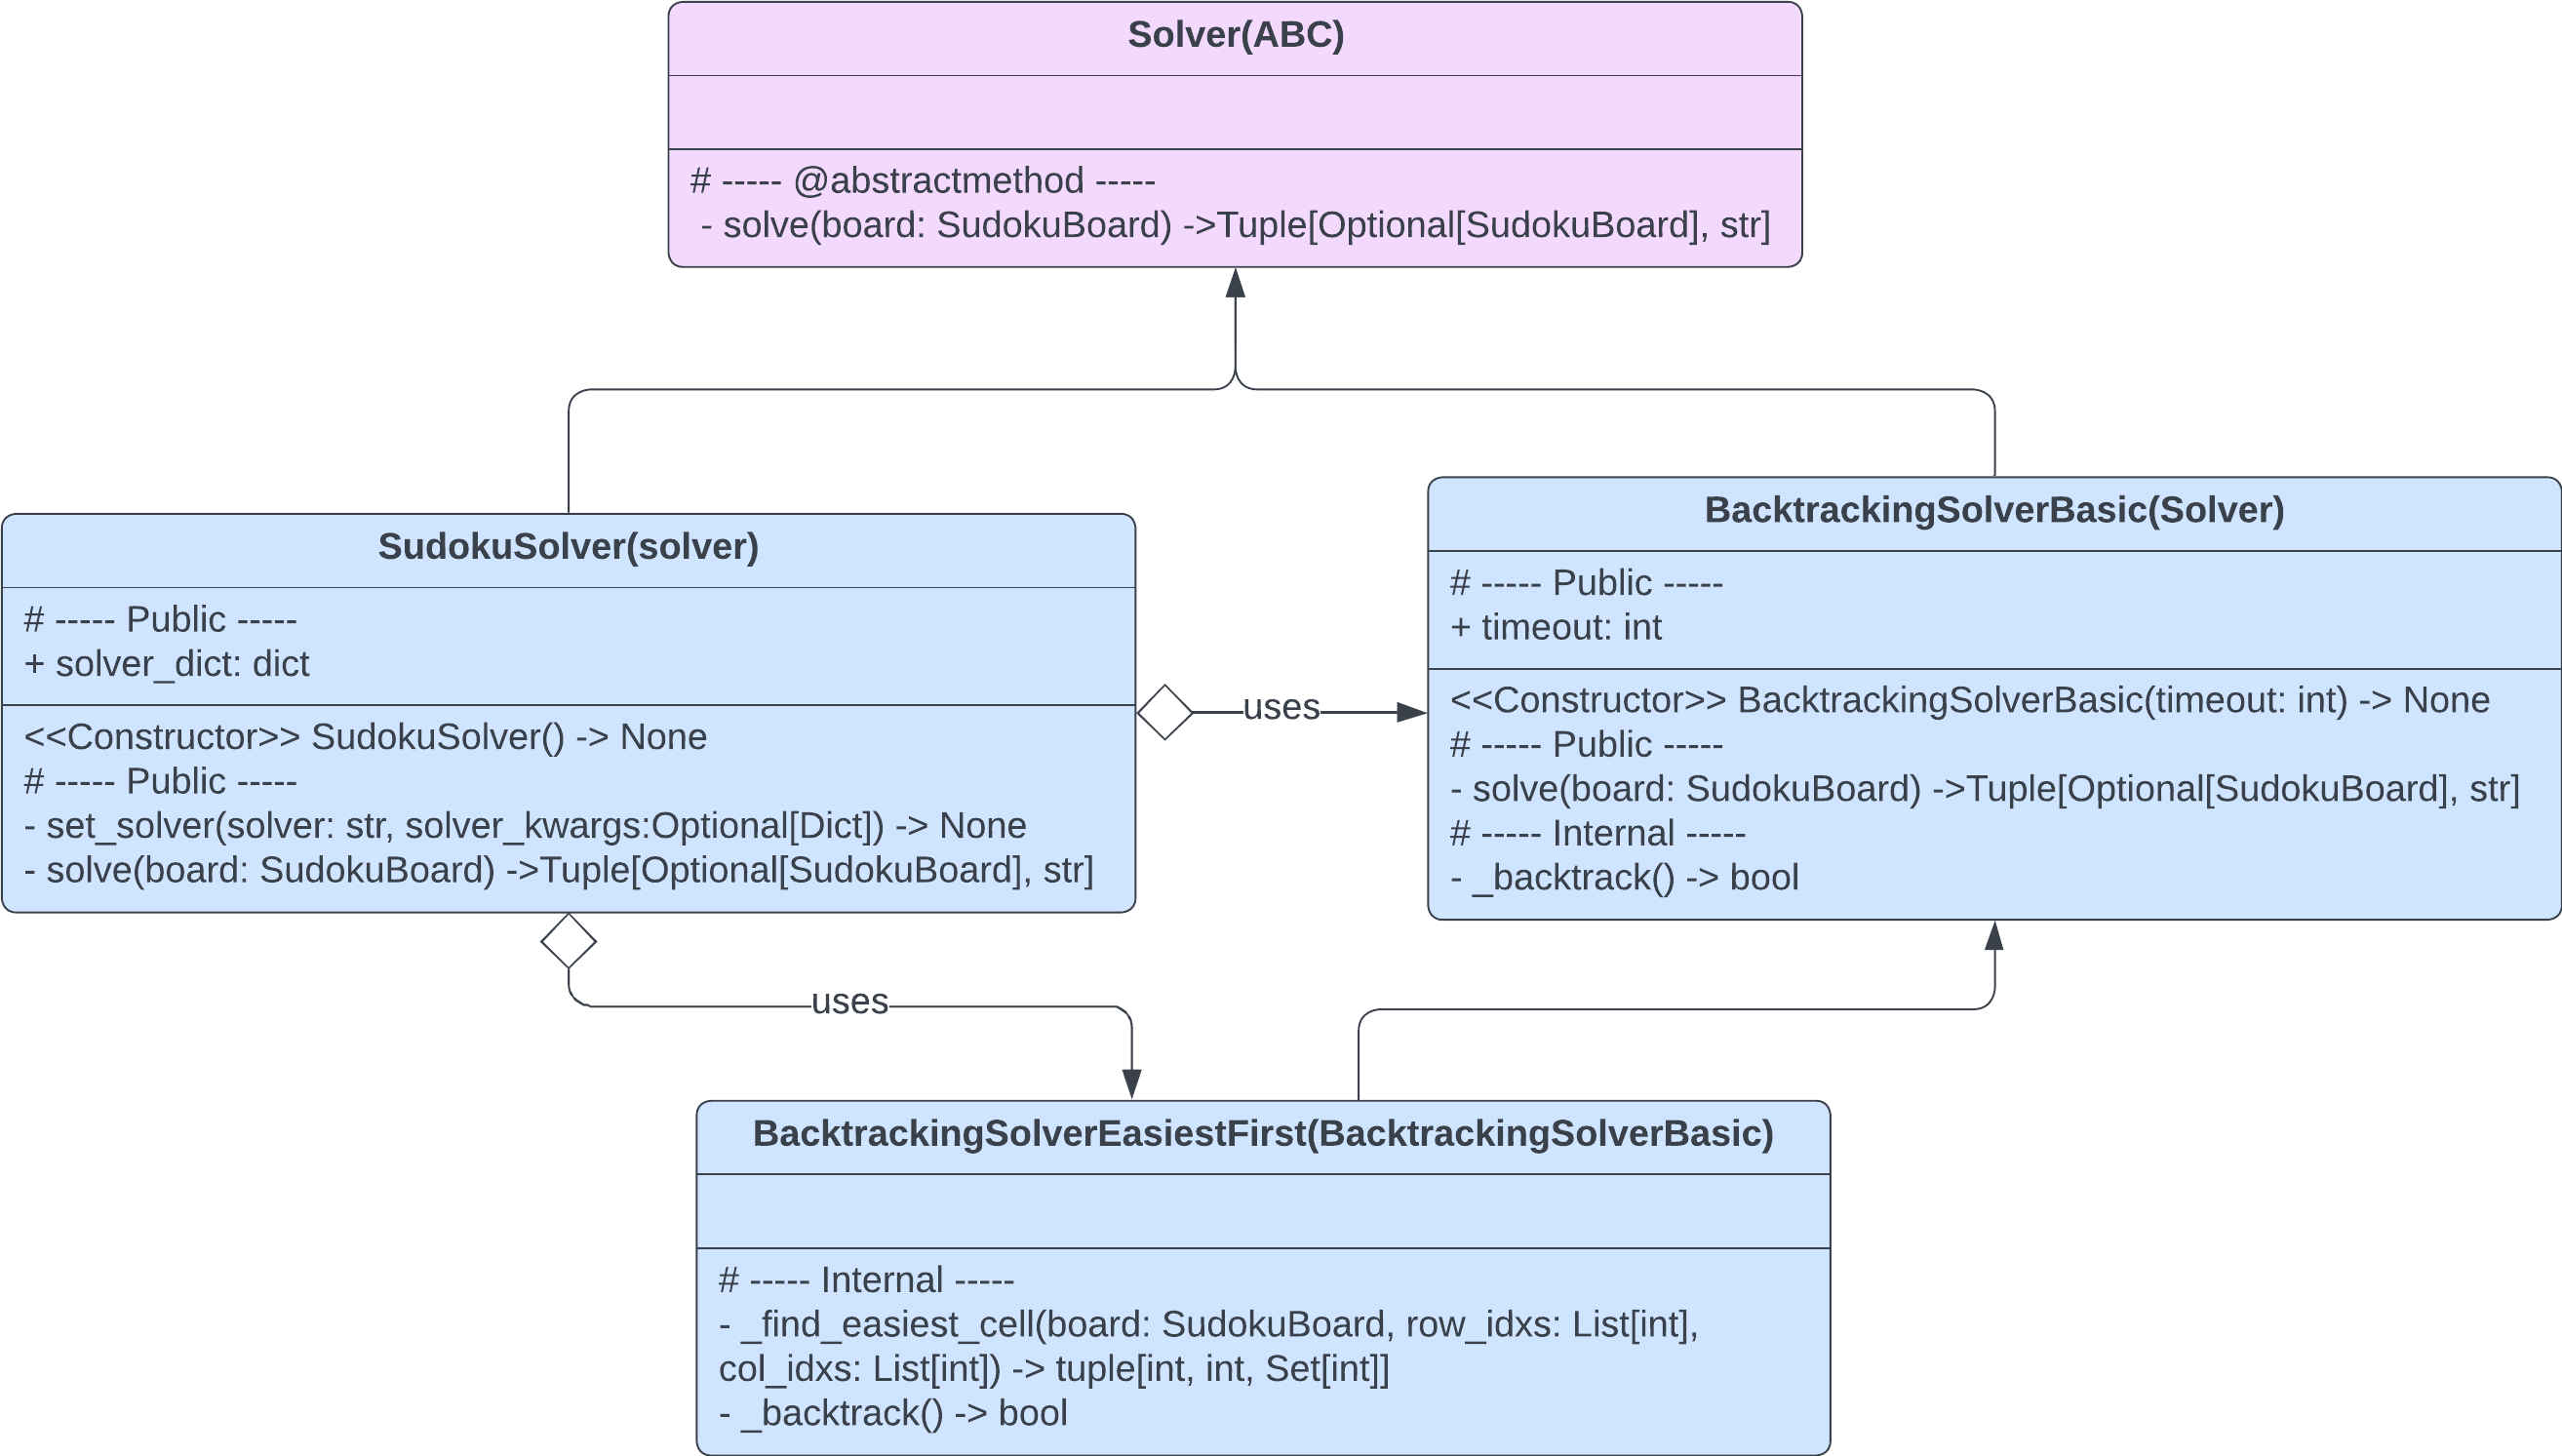
\includegraphics[width=1\textwidth]{figs/UML_sudoku_solver.png}
    \caption{UML class diagram for implementation of the SudokuSolver classes. Abstract classes are depicted in pink, concrete classes in blue. Composition relationships are indicated with arrows having a white diamond base and a solid head.}
    \label{fig:sudoku_solver_uml}
\end{figure}


\subsubsection{Limitations}
The system currently operates on a single-threaded execution model, not utilizing parallel processing which could expedite solving by simultaneously exploring multiple solution tree branches. Additionally, while flexible within the backtracking approach, the framework might not easily support radically different solving methods.

\subsection{UserIO}
\subsubsection{Scope}
The user IO is handled by the \texttt{main.py} script. This script is defined by its role as the entry point for the Sudoku solver program. The scope of this script encompasses:

\begin{enumerate}
    \item \textbf{Argument Parsing and Validation:} Interprets and validates command-line arguments for configuring the solver's operation.
    \item \textbf{Initialisation:} Sets up core components like `\texttt{SudokuFormatHandler}` and `\texttt{SudokuSolver}` based on user inputs.
    \item \textbf{Solving Process Management:} Manages the Sudoku solving flow, accommodating both single and batch operations.
    \item \textbf{Statistics and Output Handling:} Gathers and presents solving statistics, handling outputs for solved puzzles.
\end{enumerate}

\subsubsection{Design and implementation}
The \texttt{main.py} script in the Sudoku solver program is underpinned by the following design principles:

\begin{itemize}
    \item \textbf{Backend Independence:} Maintains independence from the solver and format handler backends.
    \item \textbf{User Customisation:} Allows users to define input and output formats, enabling highly customised runs.
    \item \textbf{Reproducibility:} Facilitates reproducible runs by saving statistics, including the Git commit hash and run arguments.
    \item \textbf{Robust Error Handling:} Incorporates thorough argument validation and error handling to safeguard user interaction.
    \item \textbf{Intuitive Defaults with Customization Options:} Provides sensible defaults for ease of use, alongside a range of customisable arguments for advanced users.
    \item \textbf{Dynamic Solver and Formatter Integration:} Automatically enables selection of solvers and formatters added to the Sudoku solver and format handler.
    \item \textbf{Clear Output and Feedback:} Ensures outputs are easily understandable and provides clear user feedback throughout the process.
\end{itemize}

The implementation of logic is shown as a flow chart in Figure \ref{fig:main_flowchart}.

\subsubsection{Extensibility and Limitations}
The main way in which \texttt{main.py} is currently designed to be extensible is in the integration of more complex solvers. At present, solvers can be initialised with a singular timeout parameter. However, in anticipation of future more complex solvers which require more initialisation parameters, a space for that logic has been left in the \texttt{get\_solver\_kwargs} function. This function, which currently takes as input the users arguments, can easily be designed to handle the parsing of an input configuration file. This capability paves the way for the incorporation of advanced solvers without necessitating substantial modifications to the existing codebase. 
The main limitation of main.py is that adding more output metrics like backtracking recursions, or other solver based statistics requires some plumbing work. Further, implementing parallel processing will require refactoring the code. 
\begin{figure}[H]
    \centering
    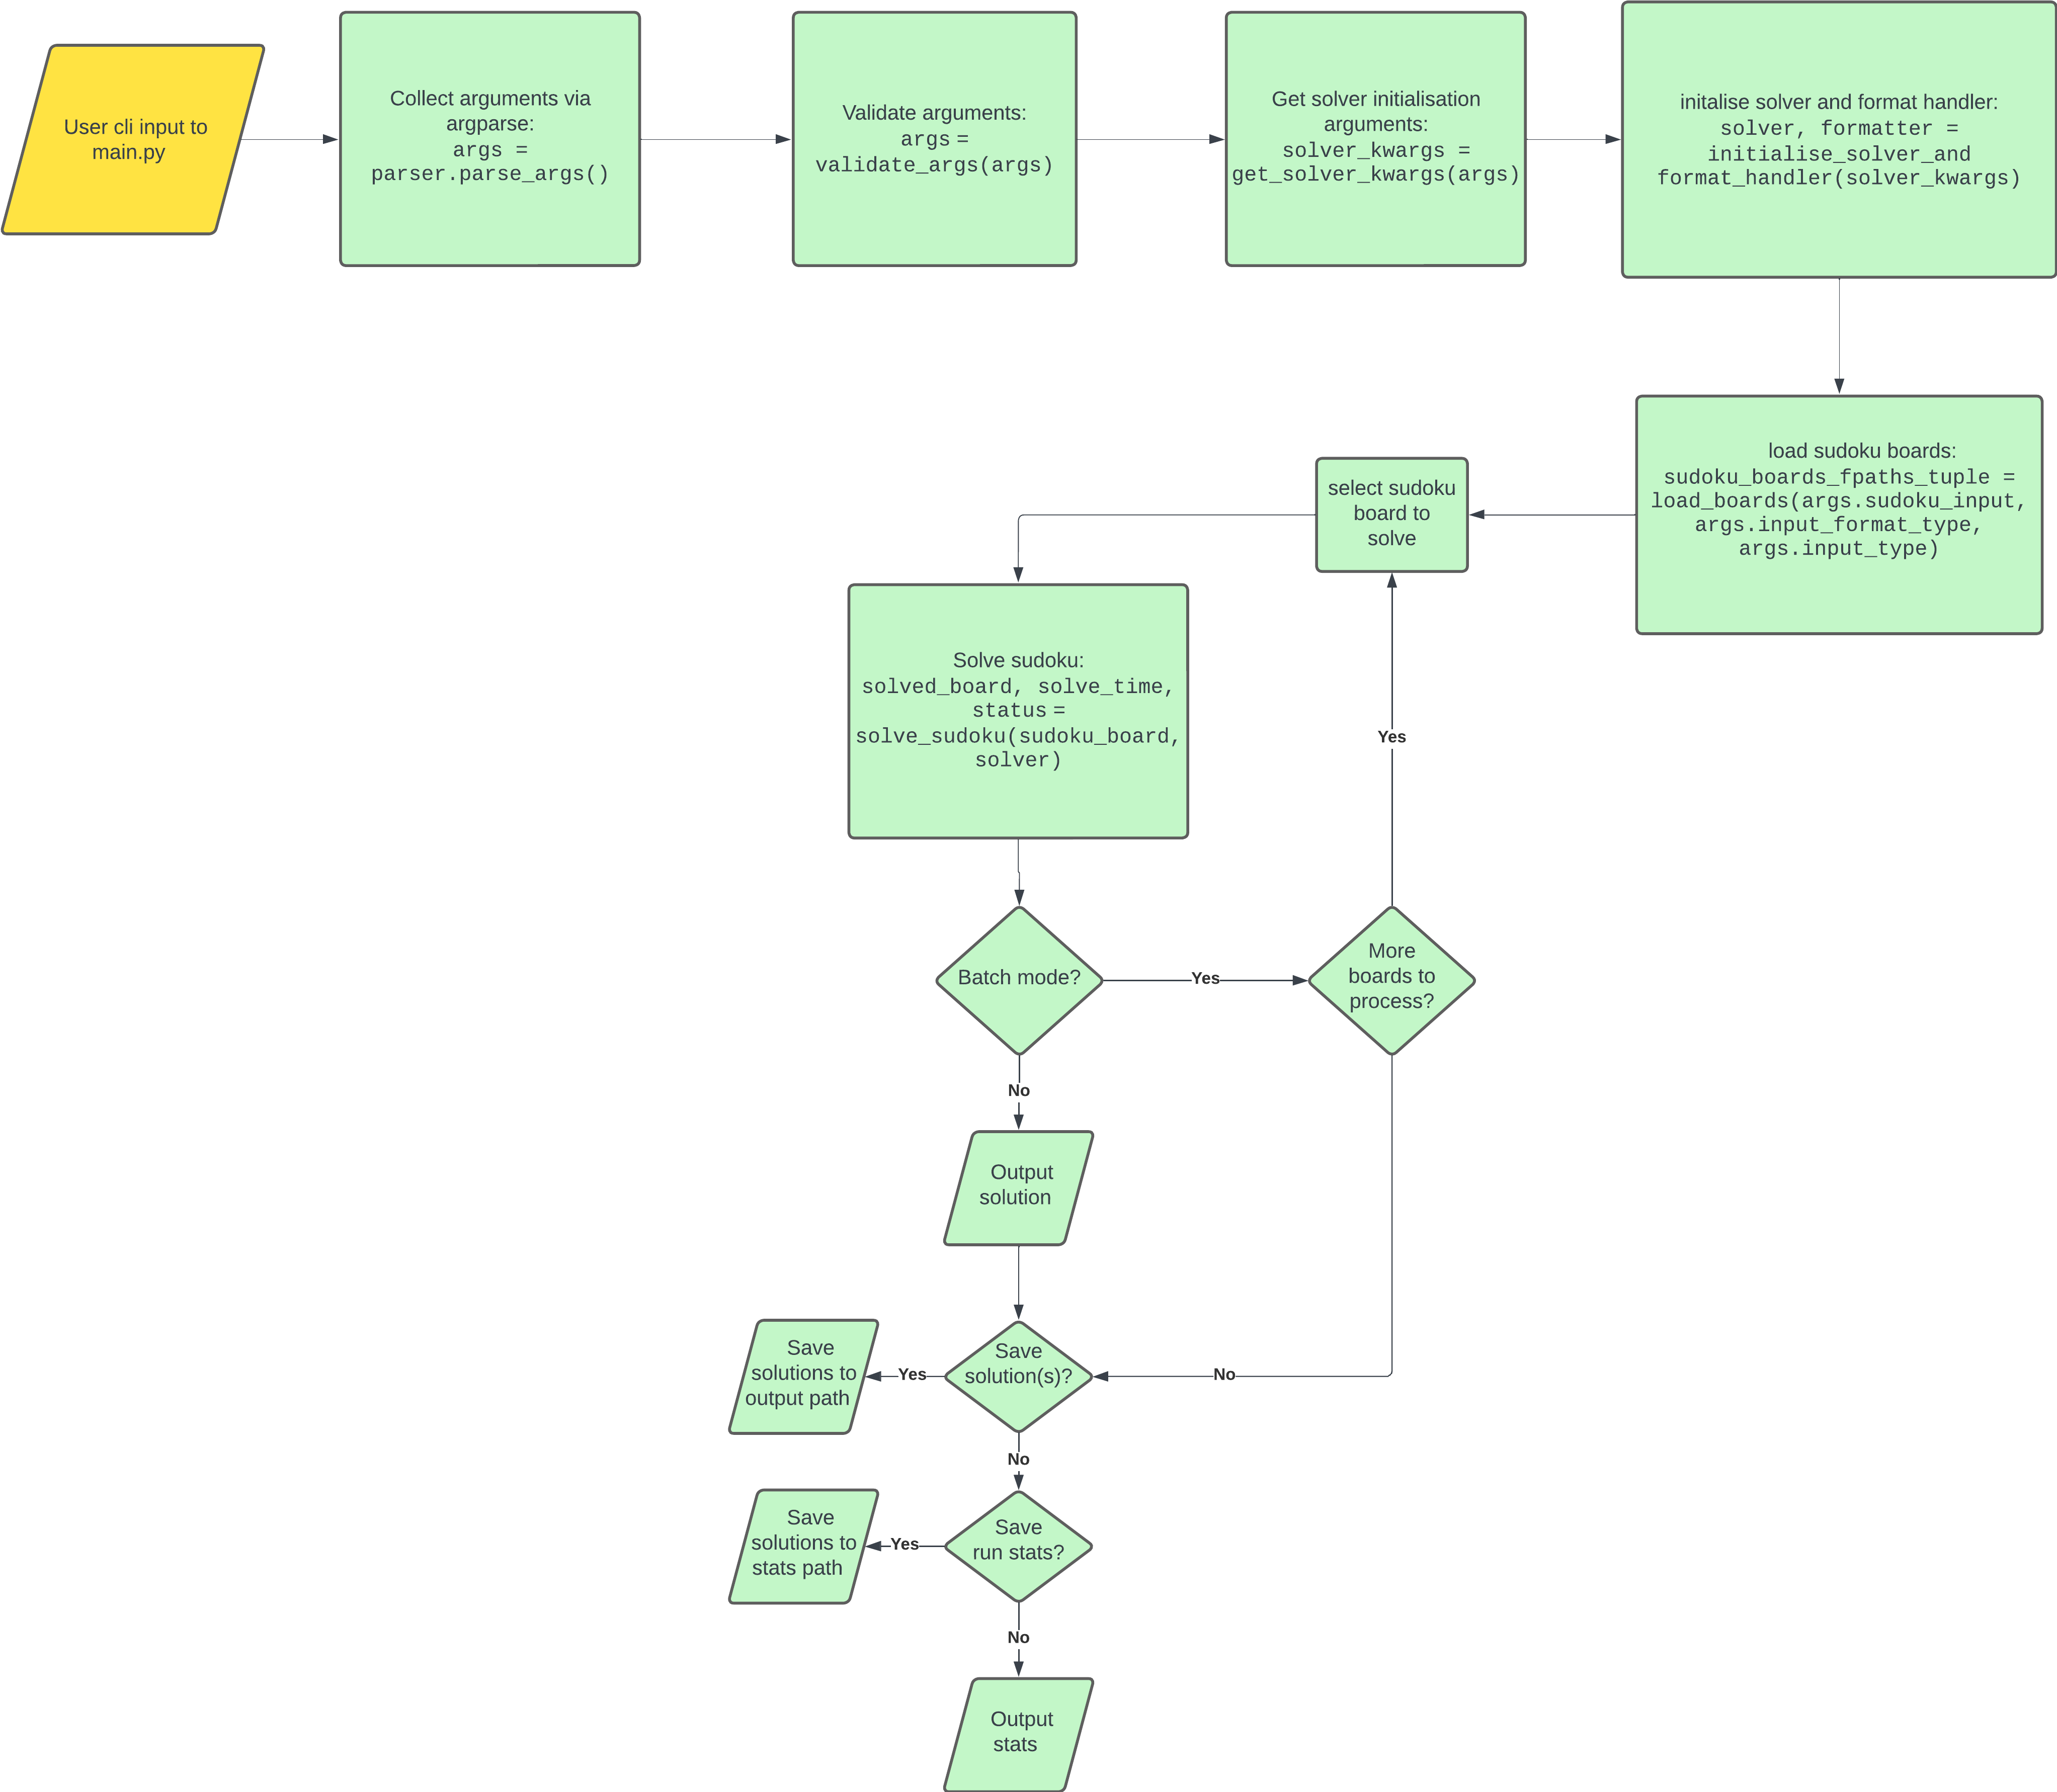
\includegraphics[width=1\textwidth]{figs/main_flowchart.png}
    \caption{Flowchart of the main.py script.}
    \label{fig:main_flowchart}
\end{figure}



\section{Profiling and optimisation}
Line profiling of the initial basic backtracking solver, implemented at the time as \texttt{BacktrackingSolver}, identified two critical functions: \texttt{check\_valid} in \texttt{SudokuBoard} and \texttt{\_backtrack} in \texttt{BacktrackingSolver}. \texttt{check\_valid} emerged as a significant bottleneck, taking 242.043 seconds, largely due to frequent calls from \texttt{\_backtrack}, which itself consumed 514.918 seconds, with 91.5\% of this time attributed to \texttt{check\_valid}. In response, the \texttt{SudokuBoard} class was restructured to store the used values of each row, column, and subgrid in class attributes as a list of sets. This change leverages the efficiency of hash tables, inherent in set data structures, for quicker lookups, instead of iterating over the board repeatedly. This adjustment reduced the execution time of \texttt{check\_valid} to just 34.9543 seconds, and the total time for \texttt{\_backtrack} was brought down to 198.044 seconds. Consequently, the time percentage of \texttt{\_backtrack} spent on \texttt{check\_valid} decreased to 73.8\%, reflecting a more evenly distributed computational effort and a significant enhancement from the original profile.


\begin{figure}[H]
    \centering
    \begin{subfigure}[b]{0.72\textwidth}
        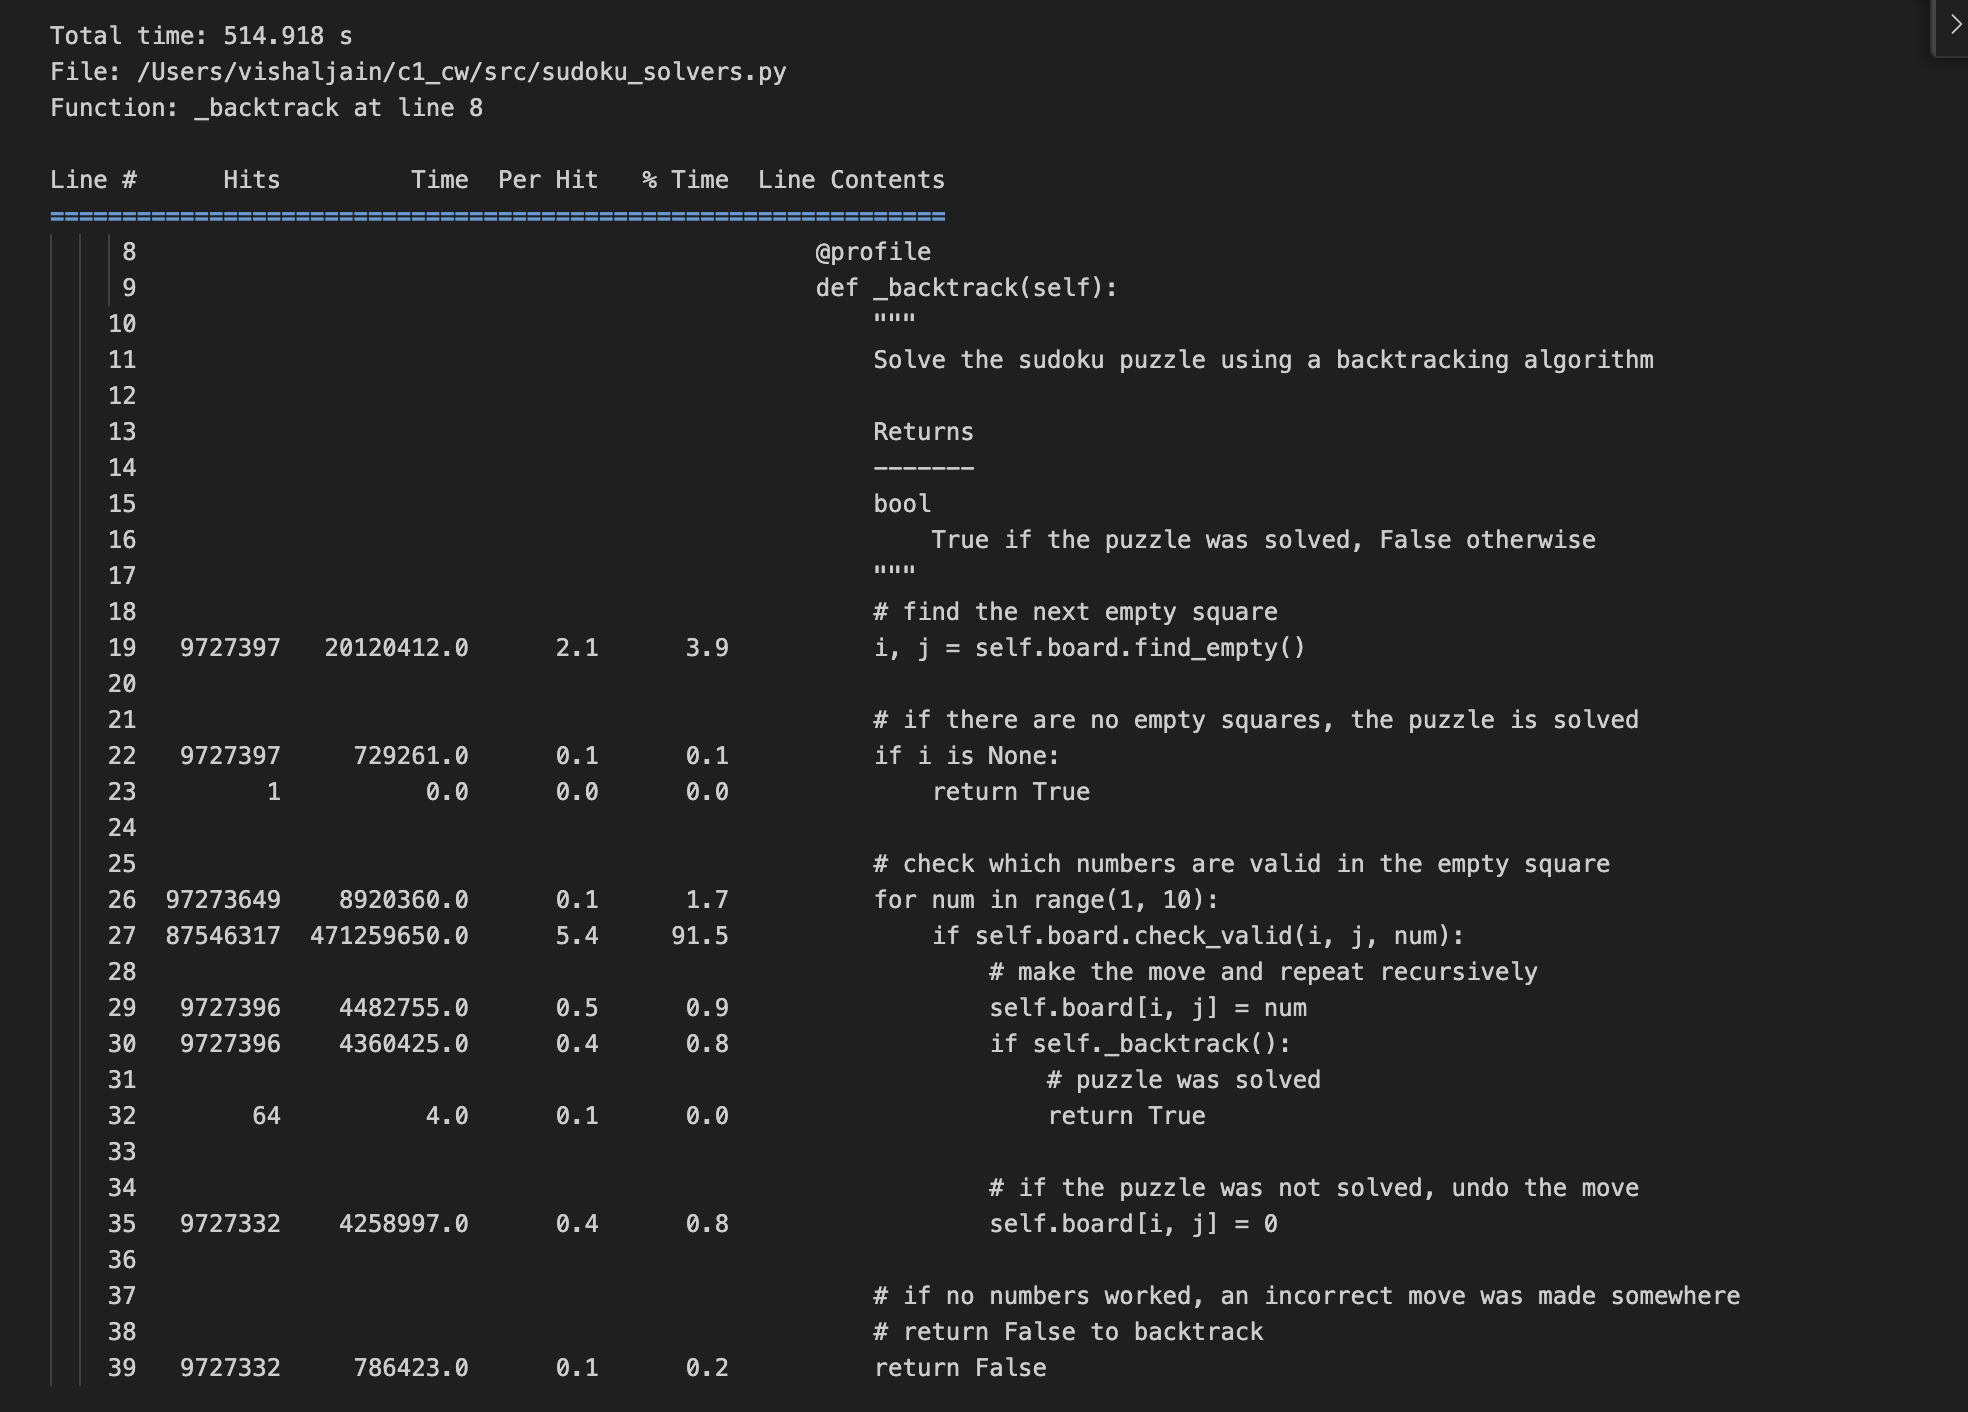
\includegraphics[width=\textwidth]{figs/bt_line_profile_before.png}
        \caption{\texttt{BacktrackingSolver.\_backtrack()} line profile results before optimisation}
        \label{fig:backtrack_before}
    \end{subfigure}
    \begin{subfigure}[b]{0.72\textwidth}
        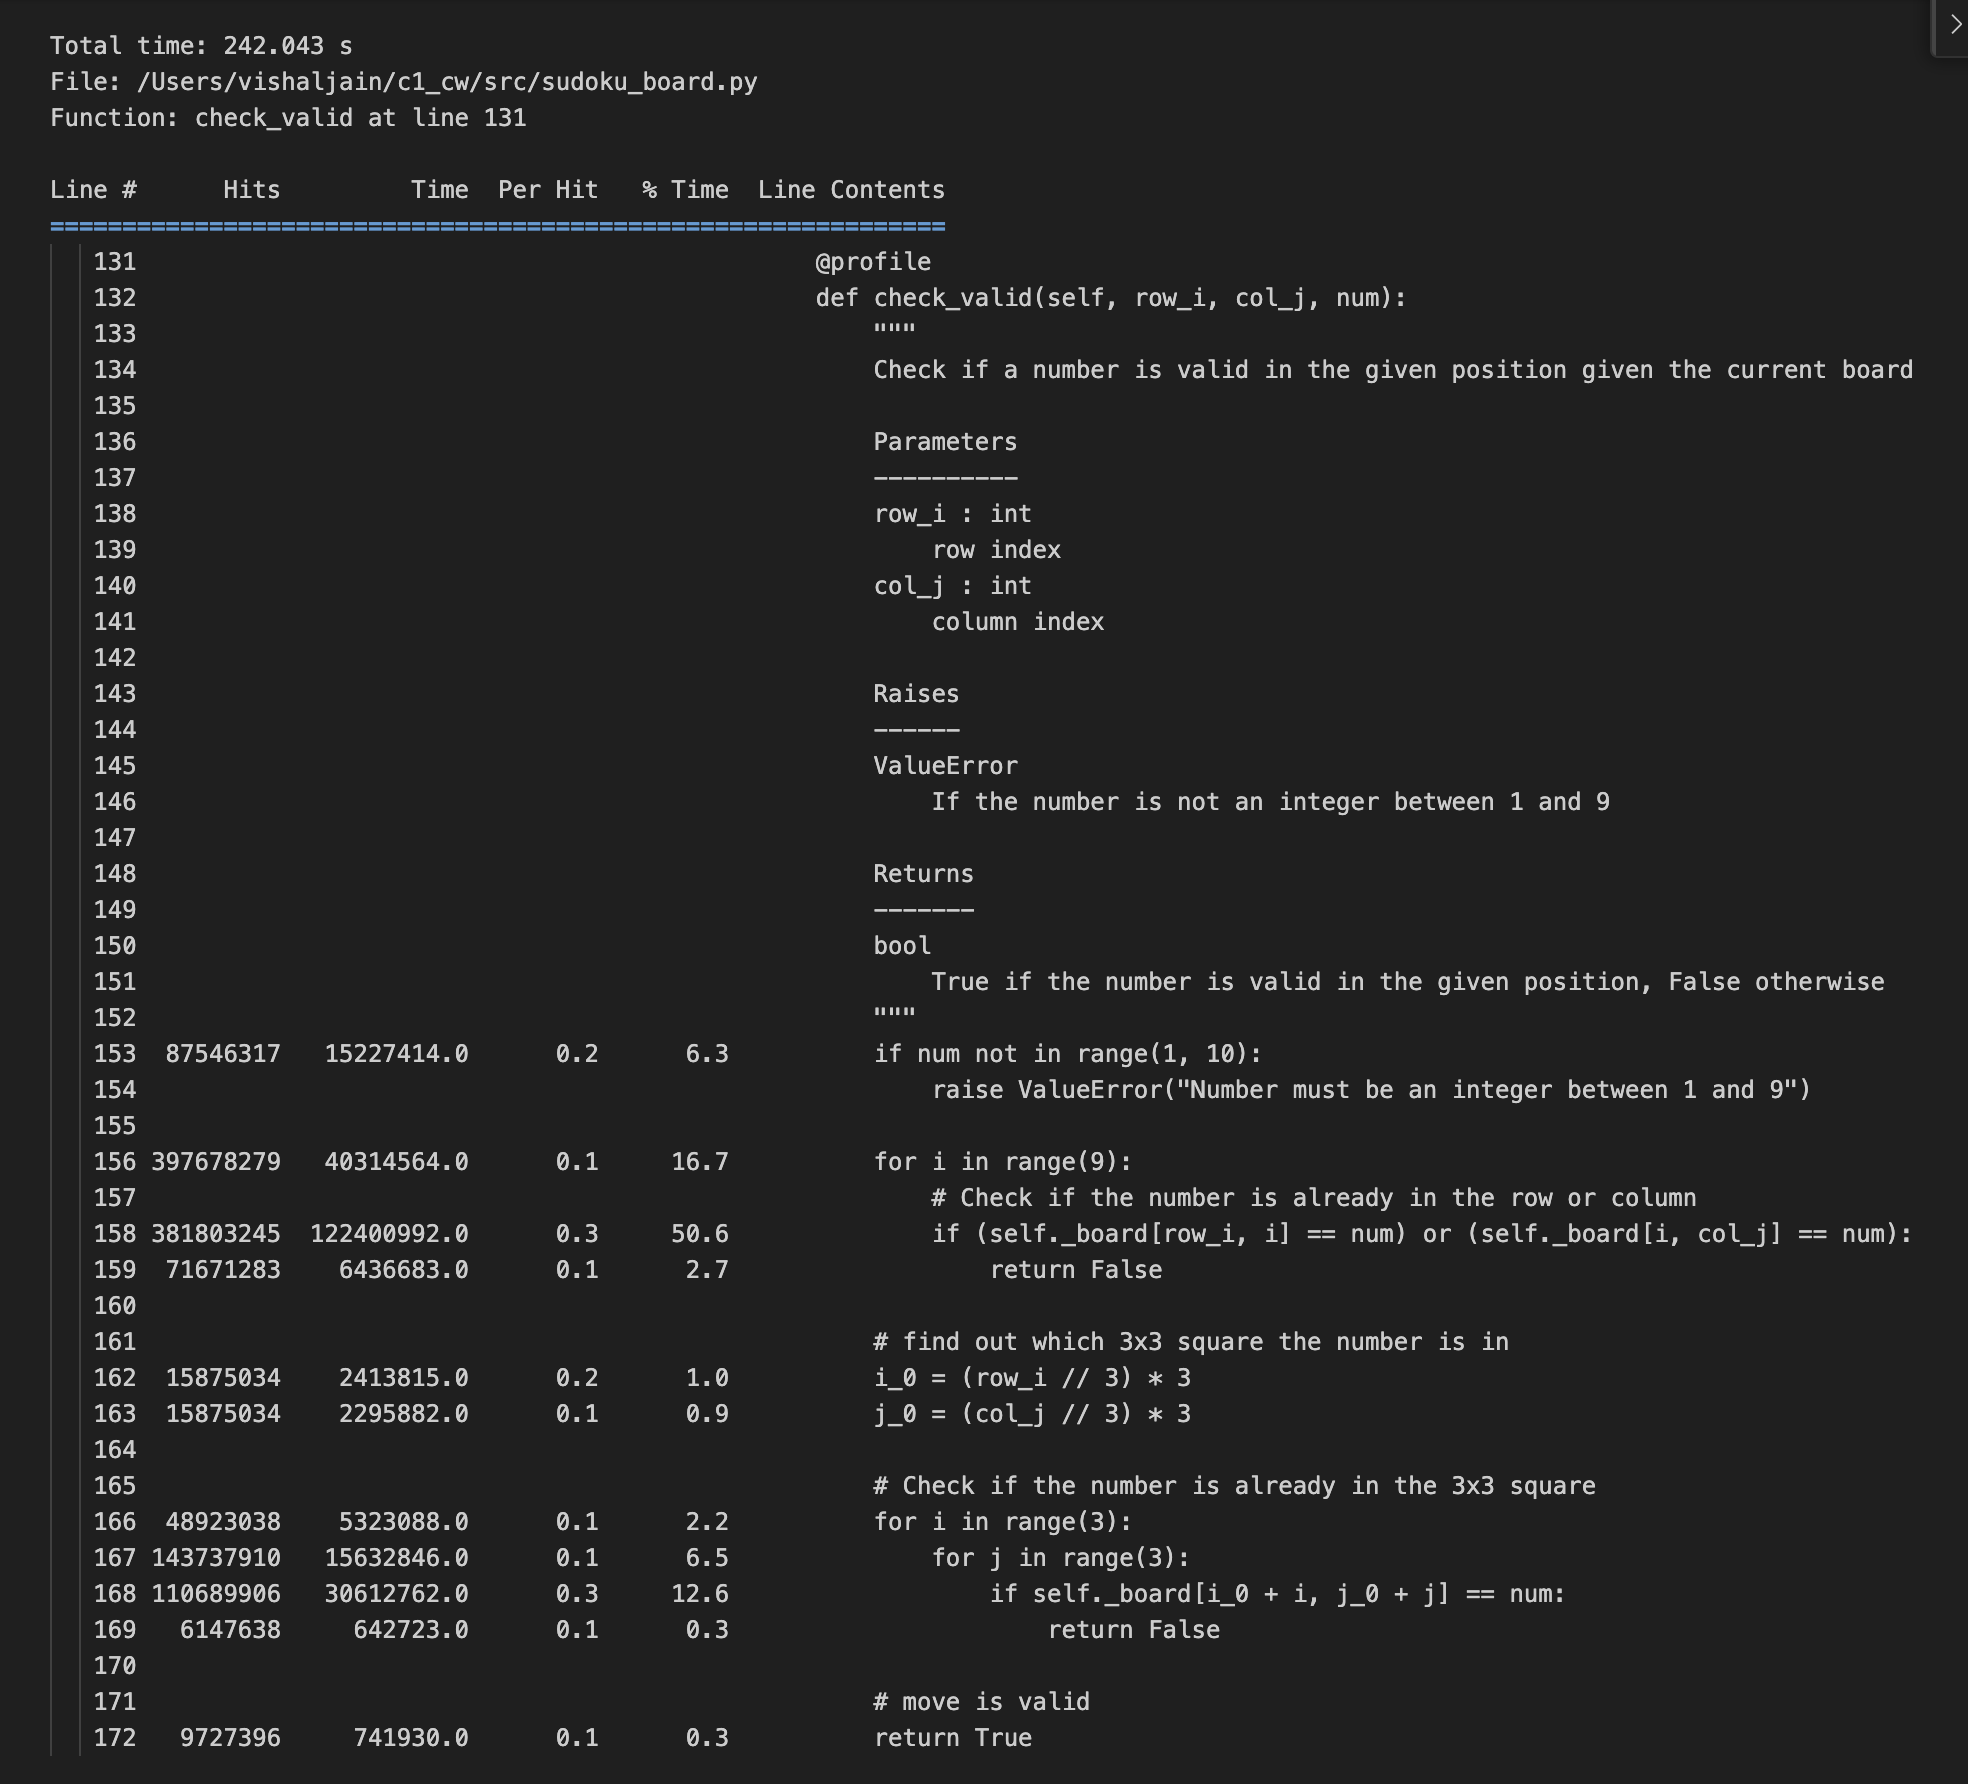
\includegraphics[width=\textwidth]{figs/check_valid_before.png}
        \caption{\texttt{SudokuBoard.check\_valid()} line profile results before optimisation}
        \label{fig:check_valid_before}
    \end{subfigure}
    \caption{Initial line profiling results before optimisation of \texttt{SudokuBoard.check\_valid} - git commit 4c1278cf}
    \label{fig:line_profiling_initial}
\end{figure}


\begin{figure}[H]
    \centering
    \begin{subfigure}[b]{0.8\textwidth}
        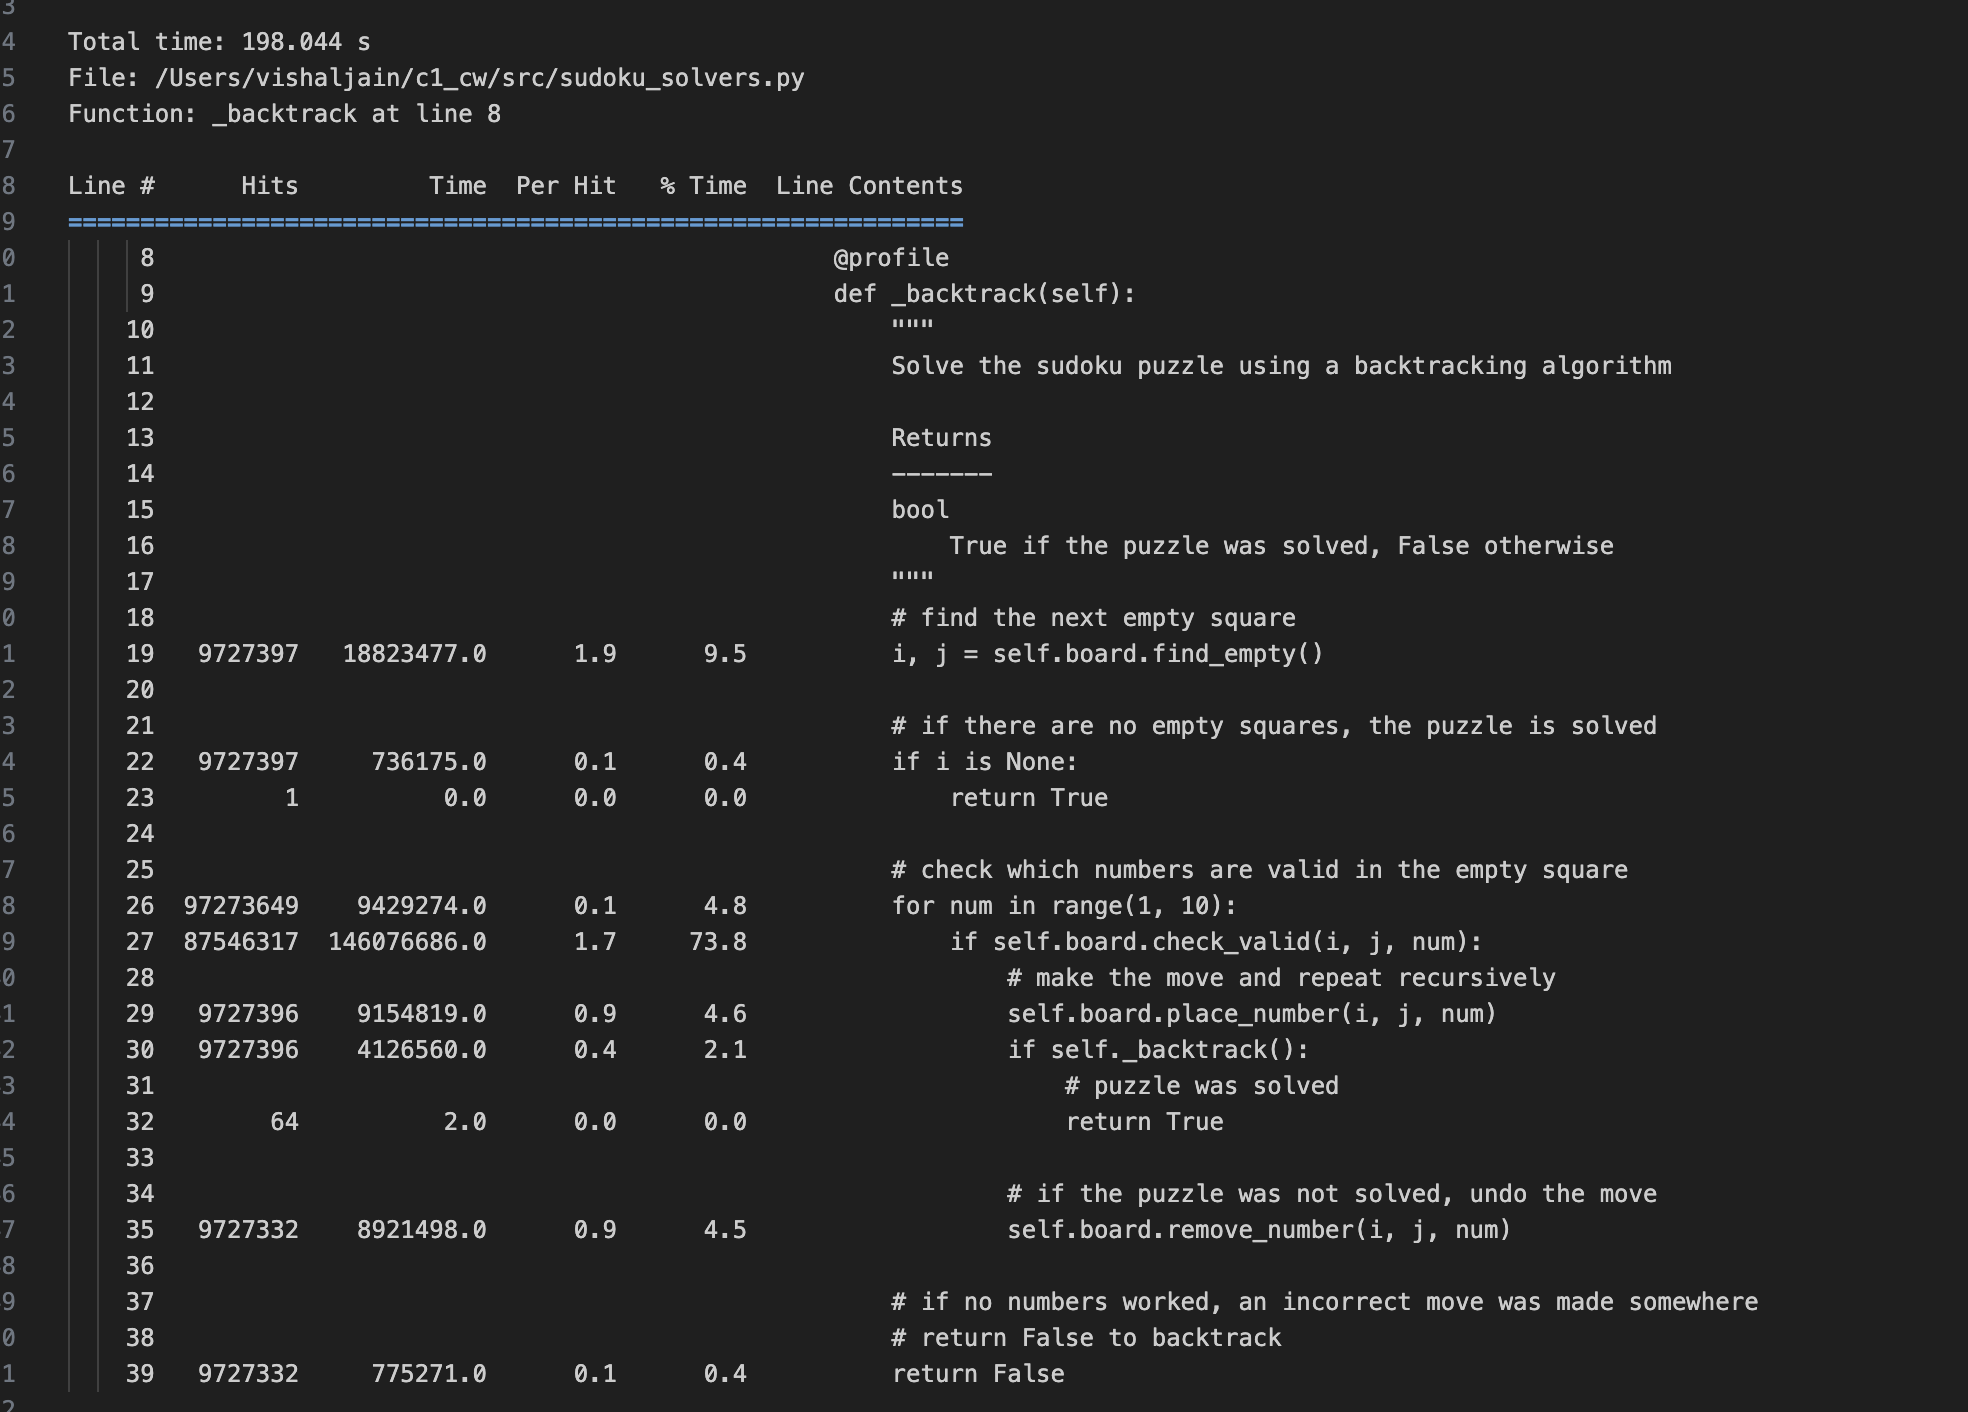
\includegraphics[width=\textwidth]{figs/bt_line_profile_after.png}
        \caption{\texttt{BacktrackingSolver.\_backtrack()} after optimisation}
        \label{fig:backtrack_after}
    \end{subfigure}
    \begin{subfigure}[b]{0.8\textwidth}
        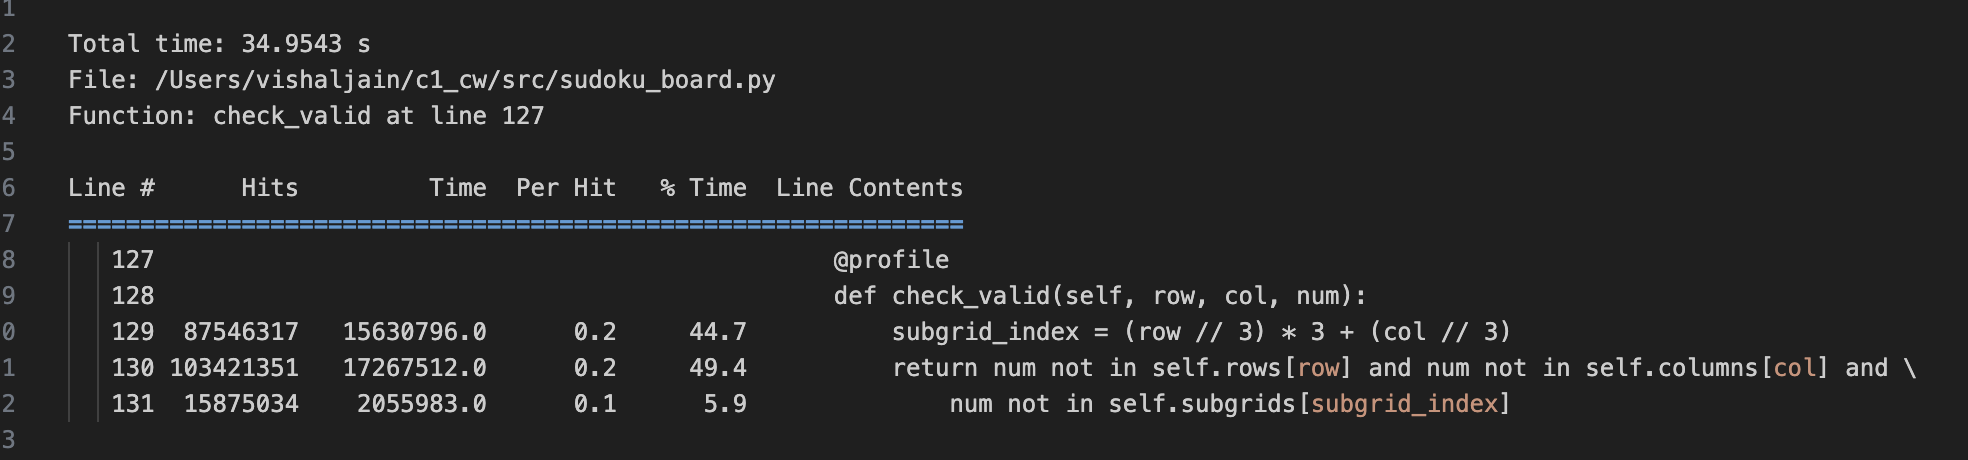
\includegraphics[width=\textwidth]{figs/check_valid_after.png}
        \caption{SudokuBoard.\texttt{check\_valid()} after optimisation}
        \label{fig:check_valid_after}
    \end{subfigure}
    \caption{Line profiling results after swapping from list based implemtation of \texttt{SudokuBoard.check\_valid} to a set based implementation - git commit c3fad894.}
    \label{fig:line_profiling_after}
\end{figure}

\section{Backtracking Solver comparison}
The performance of the basic backtracking solvers was evaluated using two distinct datasets: a set of 1 million Sudoku puzzles sourced from Kaggle \cite{kaggleDataset}, and a collection of 100 puzzles known to challenge backtracking algorithms which can be found in the repository at the path \texttt{benchmark\_board\_sets/hard\_100}. A timeout limit of 120 seconds is set to ensure completion of the solver on the hard puzzles. The results are shown in Figures \ref{fig:kaggle-million} and \ref{fig:hard-100} .

The backtracking with the easiest first heuristic is slightly slower than the basic backtracking solver on the easy puzzles due to the increased overhead of checking the number of possible values for each cell, but significantly faster on the hard puzzles. Showing the effectiveness of the heuristic in reducing the number of branches explored. Infact, two of the hard puzzles are not solved by the basic backtracking solver within the 2 minute timeout limit.

These results can be found in the \texttt{solver\_output} directory in the repository. 
\begin{figure}[H]
    \centering
    \begin{tabular}{|c|c|c|}
    \hline
    Solve Time Metric & Basic & Easiest First \\
    \hline
    Average (ms) & 0.745 & 1.30 \\
    \hline
    Median (ms) & 0.550 & 1.28 \\
    \hline
    Min (ms) & 0.273 & 1.08 \\
    \hline
    Max (ms) & 99.0 & 140 \\
    \hline
    Std (ms) & 0.725 & 0.261 \\
    \hline
    \end{tabular}
    \caption{Comparison of basic backtracking vs backtracking with easiest first heuristic performance metrics on the Kaggle million dataset.}
    \label{fig:kaggle-million}
\end{figure}

\begin{figure}[H]
    \centering
    \begin{tabular}{|c|c|c|}
    \hline
    Solve Time Metric & Basic & Easiest First \\
    \hline
    Average (s) & 7.21 & 0.674 \\
    \hline
    Median (s) & 0.953 & 0.0815 \\
    \hline
    Min (ms) & 1.38 & 2.17 \\
    \hline
    Max (s) & 107 & 11.4 \\
    \hline
    Std (s) & 15.3 & 1.87 \\
    \hline
    Timeout instances & 2 & 0 \\
    \hline
    \end{tabular}
    \caption{Performance metrics comparison: basic backtracking vs easiest first heuristic on 100 puzzles designed for challenging the backtracking algorithm.}
    \label{fig:hard-100}
\end{figure}


\section{Software Engineering Practices}

\subsection{Exception Handling}
The application includes an exceptions module \texttt{src/exceptions.py} with exceptions like \texttt{FormatError} and \texttt{TimeoutException} for targeted error scenarios. Common user errors are handled by the \texttt{main.py} script with try except blocks.
\subsection{Version control}
Git played a crucial role in version control. Branches were systematically named using feature/ and refactor/ conventions to enhance readability, while also ensuring the stability of the main branch. A release branch was used when generating the runs for the tables in figures \ref{fig:kaggle-million} and \ref{fig:hard-100} to ensure reproducibility. Commit messages focused on explaining the reason for the change as well as the change itself. A .gitignore file was used to ensure that only the necessary files were committed. 

\subsection{Unit Testing and Continuous Integration}
The development of this programme was underpinned by a test-driven approach. Where possible, unit tests were written alongside the implementation of the corresponding functionality. As the project evolved, since the core logic remained largely unchanged, the initial unit tests remained relevant and effective. Unit tests were implemented using the pytest framework. Mocking is used where necessary in conjunction with testing on sample boards located in \texttt{test/\{module\_name\}\_test\_boards}. 
The tests are run automatically on every commit through pre-commit hooks in found in the \texttt{.pre-commit-config.yaml}. A practice in line with CI/CD strategies to ensure code quality and functionality before integration. The pre-commit hooks also fix file endings, remove trailing whitespaces, ensure consistent line endings. It also ensures the python scripts are properly formatted with Black and checks for PEP8 compliance with Flake8.

\subsection{Packaging and Accessibility}
For maximum accessbility, the programme was containerised via docker which provides a lightweight and portable solution enabling consistent and reproducible deployments. The environment was created using Conda and is reproducable through the associated environment.yml file. Instructions for running the containerised application are provided in the README.md file.

\section{Conclusion}
The report details the Sudoku solver's development, highlighting problem decomposition, solution design and implementation, underpinned by software engineering principles like modularisation, defensive programming, single responsibility, and encapsulation. These practices not only deliver an effective solver but also set a foundation for future enhancements and adaptability.

\section{Appendix}
The autocomplete feature of GitHub Copilot was used whilst developing code throughout the project."
in the README.md and the report.

The specifications of the machine used for profiling and benchmarking are as follows:
2021 MacBook Pro with a 2.4 GHz 10-Core M1 Pro processor and
16GB unified memory. The 8 high performance cores operate at a clock speed of 3.2 GHz and the 2
low performance cores at 2 GHz. The operating system was macOS Ventura version 13.4.1 (22F82).

\bibliographystyle{plain}
\bibliography{mybibfile}

\end{document}

